		\begin{question}{27}{Beer-Lambert}{2}{}
            La loi de Beer-Lambert traduit l'absorption de la lumière passant à travers une solution de concentration $C[\si{\mole\per\liter}]$. Il s'agit d'une loi exponentielle définie par $I(l) = I_0\cdot 10^{-\epsilon l C}$ où $I_0$ est l'intensité de la lumière avant la solution et  $l[\si{\centi\meter}]$ la distance dans la solution. $\epsilon$ est appelé le \emph{coefficient d'extinction molaire} et traduit de la capacité d'une mole de liquide à absorber la lumière (à une longueur d'onde donnée en général). À partir des données expérimentales ci-après et sachant que la solution de bromure de potassium est concentrée à \SI{2.5}{\mole\per\liter}, quelle est la valeur de ce coefficient? On rappelle que la tangente à l'origine d'une loi exponentielle $y = A^{-\alpha x}, A = Cste.$ coupe l'axe des abscisses en $x_0 = 1/\alpha$
            \begin{figure}
              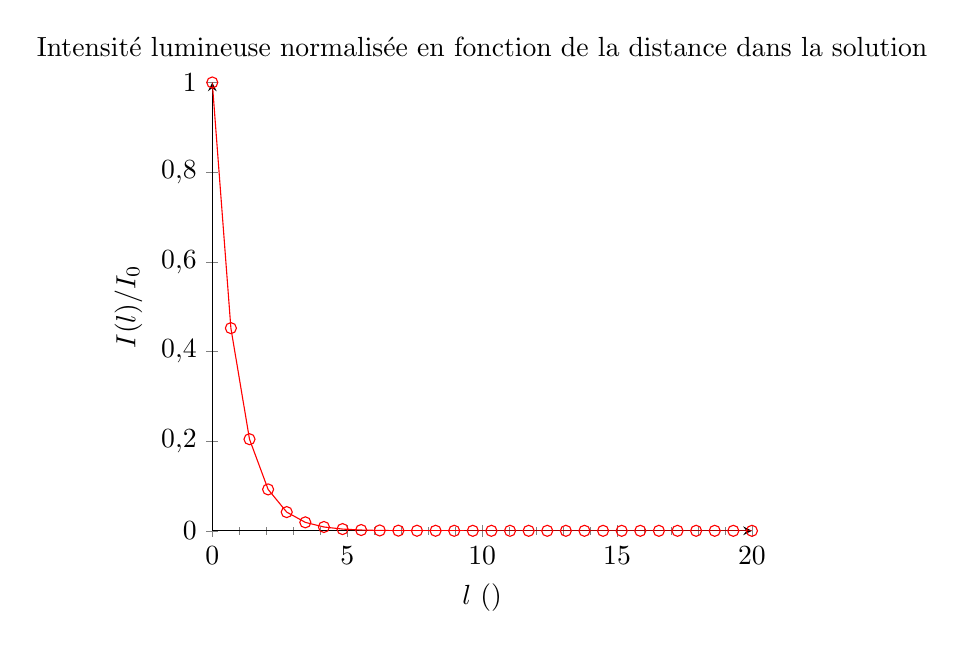
\begin{tikzpicture}
                  \begin{axis}[
                        title = {Intensité lumineuse normalisée en fonction de la distance dans la solution},
                        axis lines = left,
                        xlabel = $l$ (\si{\centi\meter}),
                        minor x tick num = 4,
                        ylabel = $I(l)/I_0$,
                        /pgf/number format/.cd,%3 lignes dessous, utiliser spacers français au lieu d'anglais.
                        use comma,
                        1000 sep={\,}
                      ]
                      %Below the red curve
                      \addplot [
                        domain=0:20,
                        samples=30,
                        color=red,
                        %/pgf/text mark = {+}, %changer le marqueur text
                        mark=o,
                      ]
                      {10^(-0.2*x*2.5)};% pour  y = a . exp(-b . x) , - a.b est la pente de la tangente à la courbe en x = 0. Cette droite coupe l'axe X en x = 1/b. Pour un même a, b indique donc la rapidité de la décroissance de la fonction.
                  \end{axis}
              \end{tikzpicture}
             \end{figure}
        \end{question}
        \begin{reponses}
            \item[false] $\epsilon \simeq \SI{2}{\liter\per\mole\per\centi\meter}$
		    \item[true] $\epsilon \simeq \SI{.2}{\liter\per\mole\per\centi\meter}$
		    \item[false] $\epsilon \simeq \SI{1}{\liter\per\mole\per\centi\meter}$
		    \item[false] $\epsilon \simeq \SI{100}{\liter\per\mole\per\centi\meter}$
		    \end{reponses}
        %%%%%%%%%%%%%%%%%%%%
        \begin{question}{27}{Beer-Lambert}{2}{}
            Considérons la loi définie par $I(x) = e^{-\alpha x}$. $\alpha$ est alors un coefficient d'extinction. À partir des données ci-après, quelle est la valeur de ce coefficient? On rappelle que la tangente à l'origine d'une loi exponentielle coupe l'axe des abscisses en $x_0 = 1/\alpha$
            \begin{figure}
              \begin{tikzpicture}
                  \begin{axis}[
                        axis lines = left,
                        xlabel = $x$,
                        minor x tick num = 4,
                        ylabel = $I(x)$,
                        /pgf/number format/.cd,%3 lignes dessous, utiliser spacers français au lieu d'anglais.
                        use comma,
                        1000 sep={\,}
                      ]
                      %Below the red curve
                      \addplot [
                        domain=0:8,
                        samples=30,
                        color=red,
                        %/pgf/text mark = {+}, %changer le marqueur text
                        mark=o,
                      ]
                      {e^(-.5*x)};% pour  y = a . exp(-b . x) , - a.b est la pente de la tangente à la courbe en x = 0. Cette droite coupe l'axe X en x = 1/b. Pour un même a, b indique donc la rapidité de la décroissance de la fonction.
                  \end{axis}
              \end{tikzpicture}
             \end{figure}
        \end{question}
        \begin{reponses}
            \item[false] $\alpha \simeq \num{5}$
		    \item[true] $\alpha \simeq \num{0.5}$
		    \item[false] $\alpha \simeq \num{1}$
		    \item[false] $\alpha \simeq \num{2}$
		    \end{reponses}
        %%%%%%%%%%%%%%%%%%%%
        \begin{question}{27}{Beer-Lambert}{3}{}
            La loi de Beer-Lambert traduit l'absorption de la lumière passant à travers une solution de concentration $C[\si{\mole\per\liter}]$. Il s'agit d'une loi exponentielle définie par $I(l) = I_0\cdot 10^{-\epsilon l C}$ où $I_0$ est l'intensité de la lumière avant la solution et  $l[\si{\centi\meter}]$ la distance dans la solution. $\epsilon$ est appelé le \emph{coefficient d'extinction molaire} et traduit de la capacité d'une mole de liquide à absorber la lumière (à une longueur d'onde donnée en général). À partir des données expérimentales ci-après et sachant que la solution de chlorure de potassium est concentrée à \SI{10}{\mole\per\liter}, quelle est la valeur de ce coefficient?
            \begin{figure}
              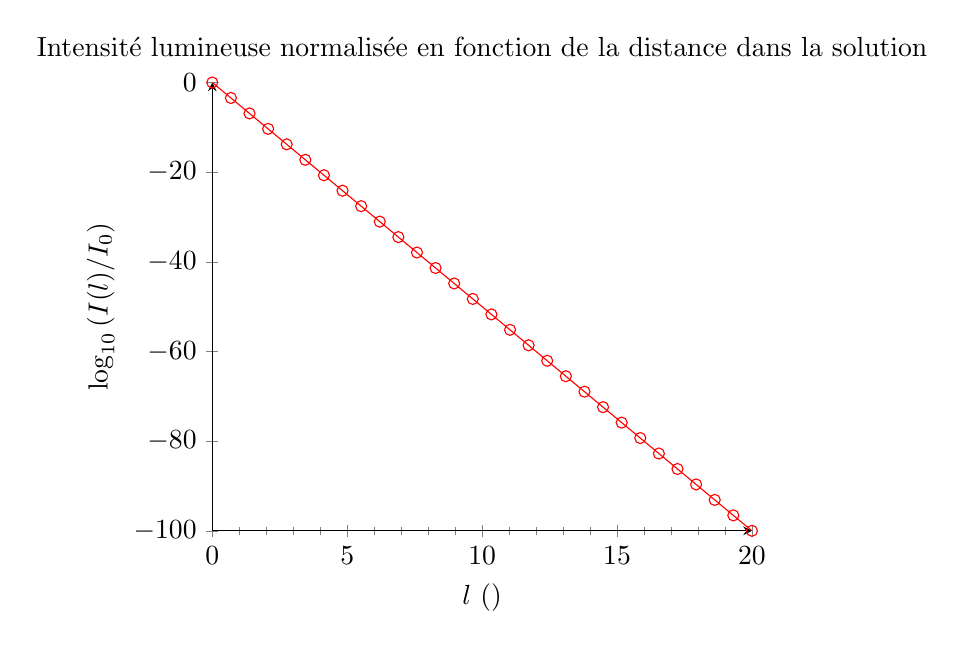
\begin{tikzpicture}
                  \begin{axis}[
                        title = {Intensité lumineuse normalisée en fonction de la distance dans la solution},
                        axis lines = left,
                        xlabel = $l$ (\si{\centi\meter}),
                        minor x tick num = 4,
                        ylabel = $\log_{10}\left(I(l)/I_0\right)$,
                        /pgf/number format/.cd,%3 lignes dessous, utiliser spacers français au lieu d'anglais.
                        use comma,
                        1000 sep={}
                      ]
                      %Below the red curve
                      \addplot [
                        domain=0:20,
                        samples=30,
                        color=red,
                        %/pgf/text mark = {+}, %changer le marqueur text
                        mark=o,
                      ]
                      {-0.5*x*10};% pour  y = a . exp(-b . x) , - a.b est la pente de la tangente à la courbe en x = 0. Cette droite coupe l'axe X en x = 1/b. Pour un même a, b indique donc la rapidité de la décroissance de la fonction.
                  \end{axis}
              \end{tikzpicture}
             \end{figure}
        \end{question}
        \begin{reponses}
            \item[false] $\epsilon \simeq \SI{5}{\liter\per\mole\per\centi\meter}$
		    \item[true] $\epsilon \simeq \SI{.5}{\liter\per\mole\per\centi\meter}$
		    \item[false] $\epsilon \simeq \SI{1}{\liter\per\mole\per\centi\meter}$
		    \item[false] $\epsilon \simeq \SI{100}{\liter\per\mole\per\centi\meter}$
	    \end{reponses}
        %%%%%%%%%%%%%%%%%%%%
		\begin{question}{27}{Beer-Lambert}{3}{}
            La loi de Beer-Lambert traduit l'absorption de la lumière passant à travers une solution de concentration $C[\si{\mole\per\liter}]$. Il s'agit d'une loi exponentielle définie par $I(l) = I_0\cdot 10^{-\epsilon l C}$ où $I_0$ est l'intensité de la lumière avant la solution et  $l[\si{\centi\meter}]$ la distance dans la solution. $\epsilon$ est appelé le \emph{coefficient d'extinction molaire} et traduit de la capacité d'une mole de liquide à absorber la lumière (à une longueur d'onde donnée en général). À partir des données expérimentales ci-après et sachant que la solution de chlorure de sodium est concentrée à \SI{6}{\mole\per\liter}, quelle est la valeur de ce coefficient? Quelle est l'intensité initiale de la lumière incidente?
        \begin{figure}
            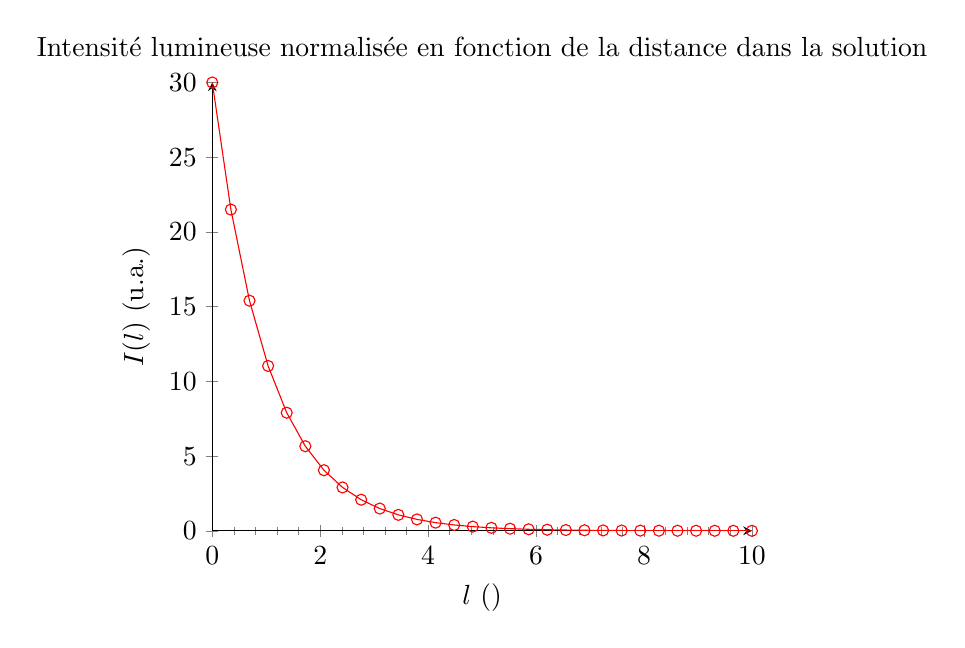
\begin{tikzpicture}
                \begin{axis}[
                        title = {Intensité lumineuse normalisée en fonction de la distance dans la solution},
                        axis lines = left,
                        xlabel = $l$ (\si{\centi\meter}),
                        minor x tick num = 4,
                        ylabel = $I(l)$ (\si{{u.a.}}),
                        /pgf/number format/.cd,%3 lignes dessous, utiliser spacers français au lieu d'anglais.
                        use comma,
                        1000 sep={}
                        ]
                    %Below the red curve
                    \addplot[
                        domain=0:10,
                        samples=30,
                        color=red,
                        %/pgf/text mark = {+}, %changer le marqueur text
                        mark=o,
                        ]
                    {30*10^(-0.07*x*6)};% pour  y = a . exp(-b . x) , - a.b est la pente de la tangente à la courbe en x = 0. Cette droite coupe l'axe X en x = 1/b. Pour un même a, b indique donc la rapidité de la décroissance de la fonction.
                \end{axis}
              \end{tikzpicture}
             \end{figure}
        \end{question}
        \begin{reponses}
            \item[false] $\epsilon \simeq \SI{6}{\liter\per\mole\per\centi\meter}$
		    \item[true] $\epsilon \simeq \SI{.07}{\liter\per\mole\per\centi\meter}$
		    \item[true] $I_0 = \SI{30}{{u.a.}}$
		    \item[false] $I_0 = \SI{16}{{u.a.}}$
	    \end{reponses}
        %%%%%%%%%%%%%%%%%%%%
		\begin{question}{27}{Beer-Lambert}{3}{}
            La loi de Beer-Lambert traduit l'absorption de la lumière passant à travers une solution de concentration $C[\si{\mole\per\liter}]$. Il s'agit d'une loi exponentielle définie par $I(l) = I_0\cdot 10^{-\epsilon l C}$ où $I_0$ est l'intensité de la lumière avant la solution et  $l[\si{\centi\meter}]$ la distance dans la solution. $\epsilon$ est appelé le \emph{coefficient d'extinction molaire} et traduit de la capacité d'une mole de liquide à absorber la lumière (à une longueur d'onde donnée en général). À partir des données expérimentales ci-après et sachant que la solution de chlorure de potassium est concentrée à \SI{10}{\mole\per\liter}, quelle est la valeur de ce coefficient?
            \begin{figure}
              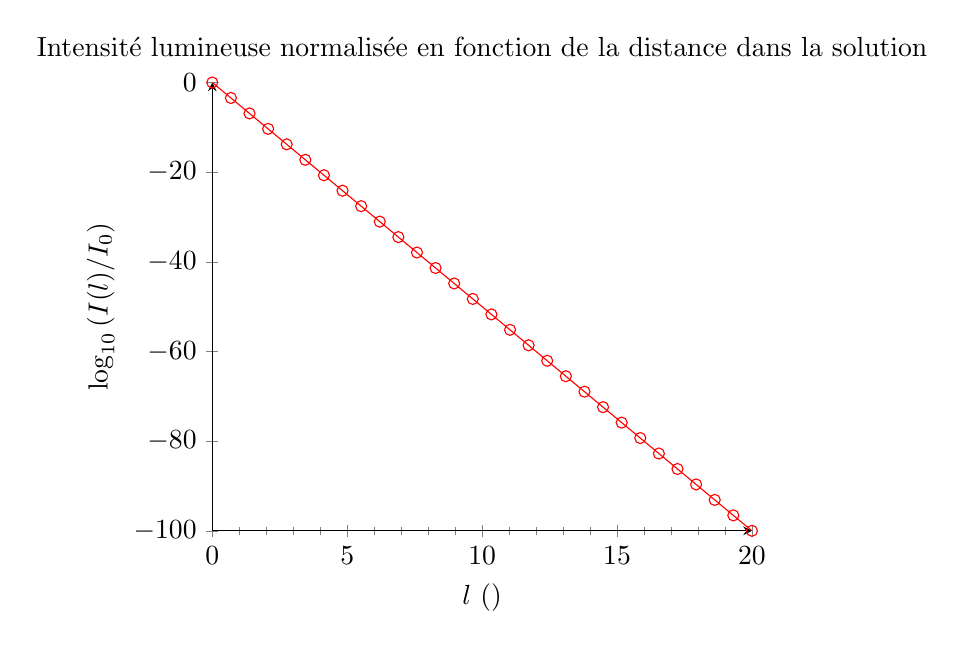
\begin{tikzpicture}
                  \begin{axis}[
                        title = {Intensité lumineuse normalisée en fonction de la distance dans la solution},
                        axis lines = left,
                        xlabel = $l$ (\si{\centi\meter}),
                        minor x tick num = 4,
                        ylabel = $\log_{10}\left(I(l)/I_0\right)$,
                        /pgf/number format/.cd,%3 lignes dessous, utiliser spacers français au lieu d'anglais.
                        use comma,
                        1000 sep={}
                      ]
                      %Below the red curve
                      \addplot [
                        domain=0:20,
                        samples=30,
                        color=red,
                        %/pgf/text mark = {+}, %changer le marqueur text
                        mark=o,
                      ]
                      {-0.5*x*10};% pour  y = a . exp(-b . x) , - a.b est la pente de la tangente à la courbe en x = 0. Cette droite coupe l'axe X en x = 1/b. Pour un même a, b indique donc la rapidité de la décroissance de la fonction.
                  \end{axis}
              \end{tikzpicture}
             \end{figure}
        \end{question}
        \begin{reponses}
            \item[false] $\epsilon \simeq \SI{5}{\liter\per\mole\per\centi\meter}$
		    \item[true] $\epsilon \simeq \SI{.5}{\liter\per\mole\per\centi\meter}$
		    \item[false] $\epsilon \simeq \SI{1}{\liter\per\mole\per\centi\meter}$
		    \item[false] $\epsilon \simeq \SI{100}{\liter\per\mole\per\centi\meter}$
	    \end{reponses}
        %%%%%%%%%%%%%%%%%%%%
